% CEFN_v2_architecture_hybrid.tex
% Hybrid architecture diagram: detailed predictor branches + clean right side
% Compile with: pdflatex CEFN_v2_architecture_hybrid.tex
\documentclass[tikz,border=8pt]{standalone}
\usepackage{tikz}
\usepackage{amsmath,amssymb}
\usetikzlibrary{positioning,fit,backgrounds,arrows.meta,calc}

% Color palette (consistent with paper figures)
\definecolor{cefnblue}{HTML}{2E86AB}
\definecolor{evo2mag}{HTML}{A23B72}
\definecolor{amorange}{HTML}{F18F01}
\definecolor{dstred}{HTML}{C73E1D}
\definecolor{gray}{HTML}{8D99AE}
\definecolor{dark}{HTML}{2B2D42}
\definecolor{lightbg}{HTML}{EDF2F4}
\definecolor{nodefill}{HTML}{F8F9FA}

\begin{document}
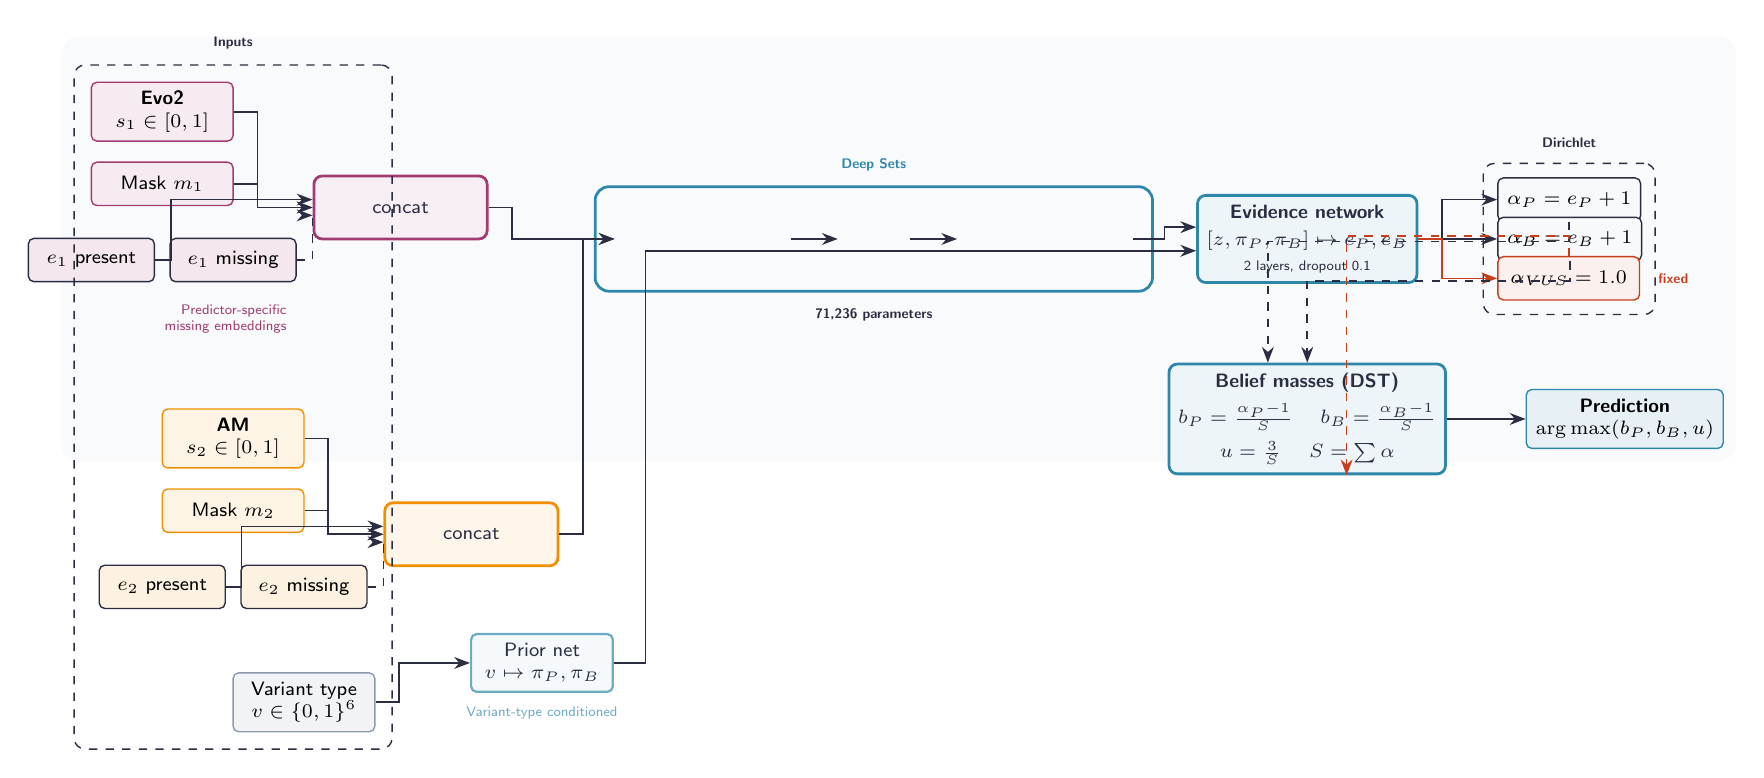
\begin{tikzpicture}[
    font=\sffamily\scriptsize,
    >=Stealth,
    thick,
    % Node styles
    input/.style={rectangle, rounded corners=2pt, draw=dark, fill=nodefill,
                  minimum width=1.8cm, minimum height=0.55cm, align=center,
                  line width=0.5pt},
    embed/.style={rectangle, rounded corners=2pt, draw=dark, fill=#1!12,
                  minimum width=1.6cm, minimum height=0.55cm, align=center,
                  line width=0.5pt},
    block/.style={rectangle, rounded corners=3pt, draw=cefnblue, fill=cefnblue!8,
                  minimum width=2.2cm, minimum height=0.8cm, align=center,
                  line width=1pt, text=dark},
    smallblock/.style={rectangle, rounded corners=2pt, draw=cefnblue!70, fill=cefnblue!5,
                       minimum width=1.8cm, minimum height=0.6cm, align=center,
                       line width=0.8pt, text=dark},
    output/.style={rectangle, rounded corners=2pt, draw=dark, fill=nodefill,
                   minimum width=1.8cm, minimum height=0.55cm, align=center,
                   line width=0.5pt},
    arrow/.style={->, line width=0.6pt, draw=dark},
    dasharrow/.style={->, line width=0.6pt, draw=dark, dashed},
    label/.style={font=\sffamily\tiny, text=gray},
]

% =============================================================================
% LEFT: PREDICTOR BRANCHES (detailed)
% =============================================================================

% --- Evo2 branch ---
\node[input, fill=evo2mag!10, draw=evo2mag] (evo2s) 
    {\textbf{Evo2}\\$s_1 \in [0,1]$};
\node[input, fill=evo2mag!10, draw=evo2mag, below=0.25cm of evo2s] (evo2m) 
    {Mask $m_1$};

% Present / absent embeddings
\node[embed=evo2mag, below=0.4cm of evo2m, xshift=-0.9cm] (evo2e) 
    {$e_1$ present};
\node[embed=evo2mag, below=0.4cm of evo2m, xshift=+0.9cm] (evo2miss) 
    {$e_1$ missing};

% Concat
\node[block, fill=evo2mag!8, draw=evo2mag, right=1.0cm of evo2m, yshift=-0.3cm] (evo2cat) 
    {concat};

% Arrows
\draw[arrow] (evo2s.east) -- ++(0.3,0) |- (evo2cat.west);
\draw[arrow] (evo2m.east) -- ++(0.3,0) |- (evo2cat.west);
\draw[arrow] (evo2e.east) -- ++(0.2,0) |- ([yshift=0.1cm]evo2cat.west);
\draw[arrow, dasharrow] (evo2miss.east) -- ++(0.2,0) |- ([yshift=-0.1cm]evo2cat.west);

% --- AlphaMissense branch ---
\node[input, fill=amorange!10, draw=amorange, below=1.6cm of evo2miss] (ams) 
    {\textbf{AM}\\$s_2 \in [0,1]$};
\node[input, fill=amorange!10, draw=amorange, below=0.25cm of ams] (amm) 
    {Mask $m_2$};

\node[embed=amorange, below=0.4cm of amm, xshift=-0.9cm] (ame) 
    {$e_2$ present};
\node[embed=amorange, below=0.4cm of amm, xshift=+0.9cm] (ammiss) 
    {$e_2$ missing};

\node[block, fill=amorange!8, draw=amorange, right=1.0cm of amm, yshift=-0.3cm] (amcat) 
    {concat};

\draw[arrow] (ams.east) -- ++(0.3,0) |- (amcat.west);
\draw[arrow] (amm.east) -- ++(0.3,0) |- (amcat.west);
\draw[arrow] (ame.east) -- ++(0.2,0) |- ([yshift=0.1cm]amcat.west);
\draw[arrow, dasharrow] (ammiss.east) -- ++(0.2,0) |- ([yshift=-0.1cm]amcat.west);

% --- Variant type input ---
\node[input, fill=gray!12, draw=gray, below=0.8cm of ammiss] (vartype) 
    {Variant type\\$v \in \{0,1\}^6$};

% --- Bracket ---
\node[fit=(evo2s)(vartype), inner sep=6pt, rounded corners=4pt,
      draw=dark, line width=0.5pt, dashed] (inputbox) {};
\node[label, above=0.06cm of inputbox.north, text=dark] {\textbf{Inputs}};

% =============================================================================
% CENTER: DEEP SETS + PRIOR + EVIDENCE
% =============================================================================

% Deep Sets
\node[block, right=1.6cm of evo2cat, yshift=-0.4cm] (phi) 
    {$\phi$ MLP};
\node[draw, circle, fill=white, minimum size=0.7cm, right=0.6cm of phi] (pool) {mean};
\node[block, right=0.6cm of pool] (rho) 
    {$\rho$ MLP\\$z \in \mathbb{R}^{128}$};

\node[fit=(phi)(rho), inner sep=7pt, rounded corners=5pt,
      draw=cefnblue, line width=1pt, fill=cefnblue!3] (dsbox) {};
\node[label, above=0.05cm of dsbox.north, text=cefnblue] 
    {\textbf{Deep Sets}};

\draw[arrow] (evo2cat.east) -- ++(0.3,0) |- (phi.west);
\draw[arrow] (amcat.east) -- ++(0.3,0) |- (phi.west);
\draw[arrow] (phi) -- (pool);
\draw[arrow] (pool) -- (rho);

% Prior
\node[smallblock, right=1.2cm of vartype, yshift=0.5cm] (prior) 
    {Prior net\\$v \mapsto \pi_P, \pi_B$};
\draw[arrow] (vartype.east) -- ++(0.3,0) |- (prior.west);
\node[label, below=0.05cm of prior.south, text=cefnblue!70] {Variant-type conditioned};

% Evidence
\node[block, right=0.8cm of rho, minimum width=2.6cm, minimum height=1.0cm] (evidence) 
    {\textbf{Evidence network}\\[2pt]
     $[z, \pi_P, \pi_B] \mapsto e_P, e_B$\\[1pt]
     \tiny 2 layers, dropout 0.1};

\draw[arrow] (rho.east) -- ++(0.4,0) |- ([yshift=0.15cm]evidence.west);
\draw[arrow] (prior.east) -- ++(0.4,0) |- ([yshift=-0.15cm]evidence.west);

% =============================================================================
% RIGHT: DIRICHLET + BELIEF + PREDICTION
% =============================================================================

% Dirichlet
\node[output, right=1.0cm of evidence, yshift=0.5cm] (alphaP) 
    {$\alpha_P = e_P + 1$};
\node[output, right=1.0cm of evidence, yshift=0cm] (alphaB) 
    {$\alpha_B = e_B + 1$};
\node[output, fill=dstred!8, draw=dstred, right=1.0cm of evidence, yshift=-0.5cm] (alphaV) 
    {$\alpha_{VUS} = 1.0$};

\node[fit=(alphaP)(alphaV), inner sep=5pt, rounded corners=4pt,
      draw=dark, line width=0.5pt, dashed] (dirbox) {};
\node[label, above=0.06cm of dirbox.north, text=dark] {\textbf{Dirichlet}};
\node[label, right=0.1cm of alphaV.east, text=dstred] {\textbf{fixed}};

\draw[arrow] (evidence.east) -- ++(0.3,0) |- (alphaP.west);
\draw[arrow] (evidence.east) -- ++(0.3,0) |- (alphaB.west);
\draw[arrow, draw=dstred] (evidence.east) -- ++(0.3,0) |- (alphaV.west);

% Belief
\node[block, below=1.0cm of evidence, minimum width=3.4cm, minimum height=1.0cm] (belief) 
    {\textbf{Belief masses (DST)}\\[3pt]
     $b_P = \frac{\alpha_P - 1}{S}$ \quad
     $b_B = \frac{\alpha_B - 1}{S}$\\[3pt]
     $u = \frac{3}{S}$ \quad
     $S = \sum \alpha$};

\draw[arrow, dasharrow] (alphaP.south) -- ++(0,-0.25) -| ([xshift=-0.5cm]belief.north);
\draw[arrow, dasharrow] (alphaB.south) -- ++(0,-0.25) -| (belief.north);
\draw[arrow, dasharrow, draw=dstred] (alphaV.north) -- ++(0,0.25) -| ([xshift=0.5cm]belief.south);

% Prediction
\node[output, fill=cefnblue!12, draw=cefnblue, right=1.0cm of belief] (pred) 
    {\textbf{Prediction}\\$\arg\max(b_P, b_B, u)$};

\draw[arrow] (belief) -- (pred);

% =============================================================================
% ANNOTATIONS
% =============================================================================
\node[label, below=0.08cm of dsbox.south, text=dark] 
    {\textbf{71,236 parameters}};
\node[label, below=0.15cm of evo2miss.south east, anchor=north east, text=evo2mag, align=right] 
    {Predictor-specific\\missing embeddings};

% =============================================================================
% BACKGROUND
% =============================================================================
\begin{scope}[on background layer]
    \fill[lightbg, rounded corners=6pt, opacity=0.4]
        ($(inputbox.north west)+(-0.15,0.35)$) rectangle
        ($(pred.south east)+(0.15,-0.15)$);
\end{scope}

\end{tikzpicture}
\end{document}
